\section{Experiments}
\label{sec:experiments}

\begin{figure}[t!]
\begin{center}
% left lower right upper
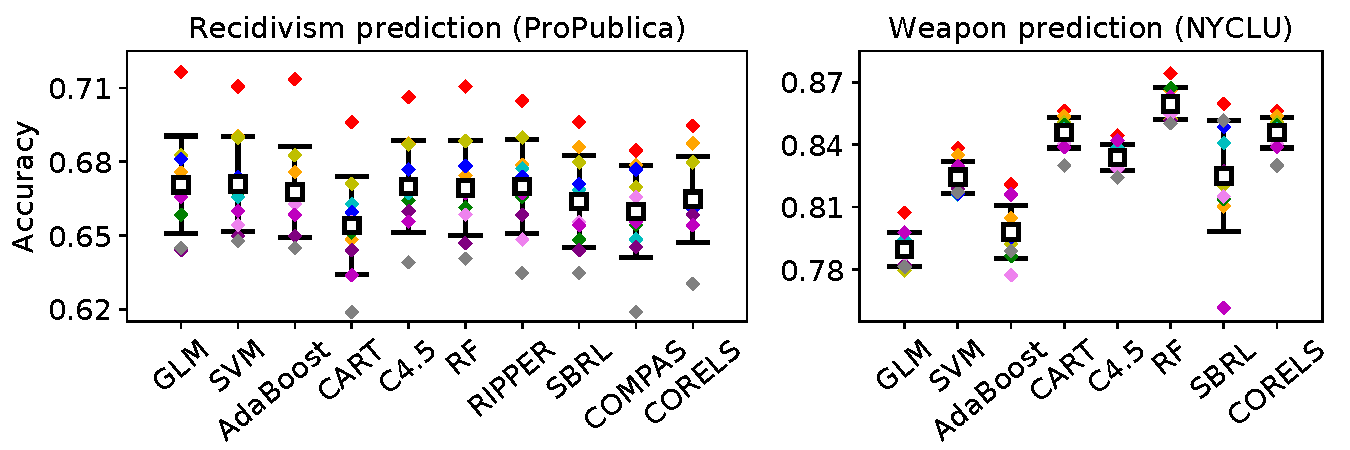
\includegraphics[trim={8mm, 10mm, 15mm, 5mm},
width=0.47\textwidth]{figs/compare-compas-weapon.pdf}
\end{center}
\caption{Test accuracy means (white squares),
standard deviations (error bars),
and values (colors correspond to folds).
For CORELS, ${\Reg = 0.005}$ (left) and ${\Reg = 0.01}$ (right).
}
\label{fig:comparison}
\end{figure}

\begin{figure}[t!]
\begin{center}
% left lower right upper
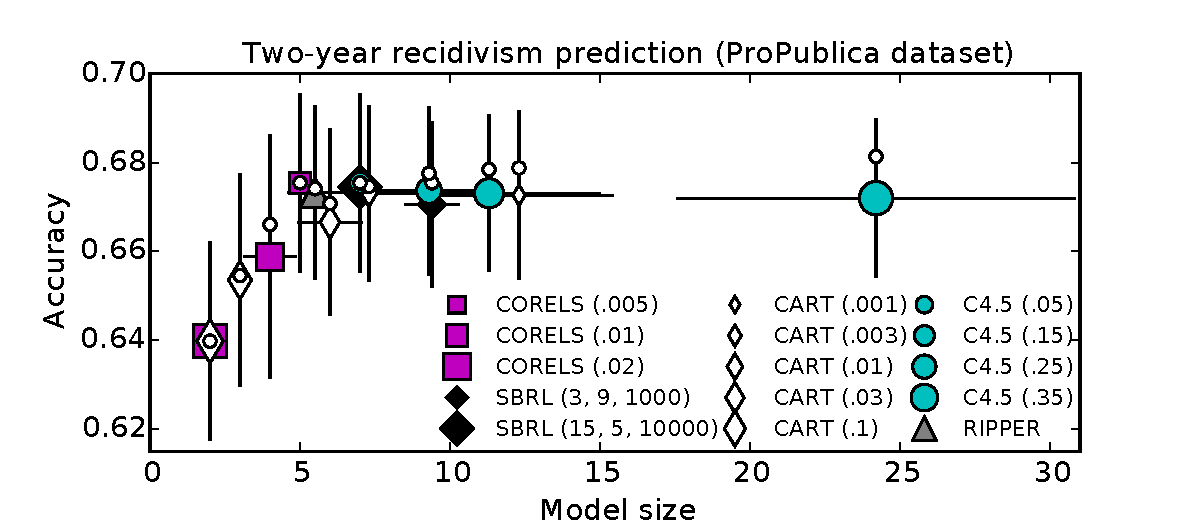
\includegraphics[trim={12mm, 7mm, 24mm, 10mm}, width=0.44\textwidth]{figs/compas-sparsity-training.pdf}
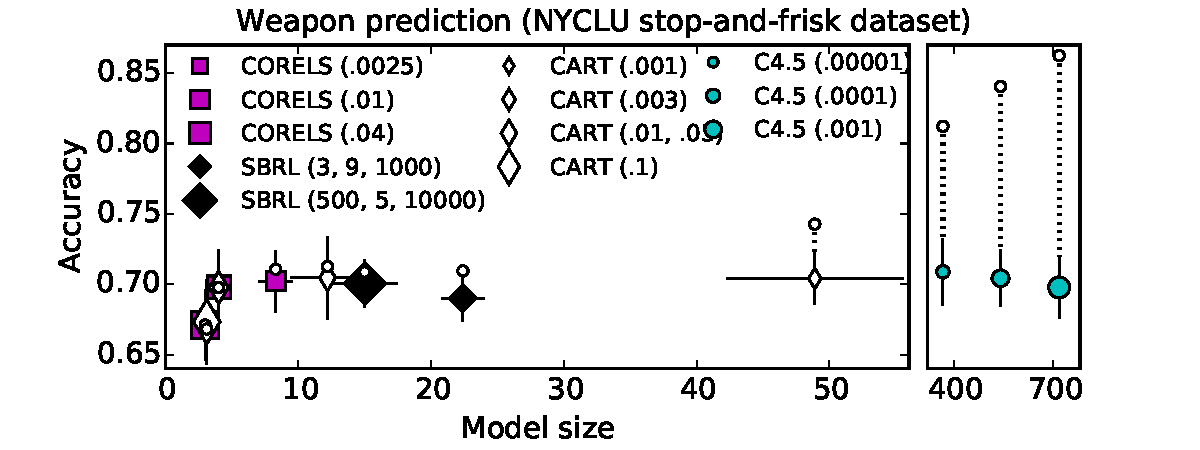
\includegraphics[trim={15mm, 12mm, 24mm, 1mm}, width=0.44\textwidth]{figs/frisk-sparsity-training-c45.pdf}
\end{center}
\caption{Training and test accuracy as a function of model size.
%
For CORELS, CART, and C4.5, we vary the regularization parameter~$\Reg$
and complexity parameters~$cp$ and~$C$, respectively.
% and are indicated within parentheses in the legend.
%
Legend markers and error bars indicate means and standard deviations,
respectively, of test accuracy across cross-validation folds.
%
Small circles mark training accuracy means.
%
Top:  %Two-year recidivism prediction for the ProPublica COMPAS dataset.
ProPublica dataset.
%
None of the models exhibit significant overfitting.
%mean training accuracy never exceeds mean test accuracy
%by more than about 0.01.
%
Bottom:  %Weapon prediction for the NYCLU stop-and-frisk dataset.
NYCLU dataset.
%
%Only CART with ${cp = 0.001}$ significantly overfits.
%
%We do not depict C4.5, which finds large models (${>100}$ leaves)
%and dramatically overfits for all tested parameters.
CART with ${cp = 0.001}$ significantly overfits, as does C4.5,
which finds large models and dramatically overfits for all tested parameters.
%
Note the broken horizontal axis and change in scale.
}
\label{fig:sparsity}
\end{figure}

% CART implementation in R's rpart
% C4.5 = J48 in RWeka
% RIPPER in R's caret

Our experimental analysis addresses four questions:
(1)~How does CORELS' accuracy and model size compare to that of other algorithms?
(2)~How rapidly do the objective value and its lower bound converge, for different values of~$\Reg$?
(3)~How much does each of the implementation optimizations contribute to CORELS' performance?
(4)~How rapidly does CORELS prune the search space?
We present additional empirical results and further implementation and data processing details
in a long version of this report~\citep{AngelinoLaAlSeRu17}.

All timed results ran on a server with two Intel Xeon E5-2699~v4
(55~MB cache, 2.20~GHz) processors and 756~GB RAM.
%
Except where we mention a memory constraint, all experiments
can run comfortably on smaller machines, \eg a laptop with 16GB~RAM.

We focus on two problems:
%using the ProPublica dataset~\citep{LarsonMaKiAn16} to predict two-year recidivism
%and using the NYCLU 2014 stop-and-frisk dataset~\citep{nyclu:2014} to predict
%whether a weapon will be found on a stopped individual who is frisked or searched.
(1)~Predicting which individuals in the ProPublica COMPAS dataset~\citep{LarsonMaKiAn16}
recidivate within two years (${N = 7,215}$).
Our rule mining procedure yields ${M = 156}$ single- and two-clause antecedents.
%
(2)~Using the NYCLU 2014 stop-and-frisk dataset~\citep{nyclu:2014}
to predict whether a weapon will be found on a stopped individual who is frisked or searched.
We identify a subset of 29,595 records for stopped individuals who were frisked and/or searched.
Of these, criminal possession of a weapon was identified in about 5\% of instances,
thus we resampled due to class imbalance.
In the first two subsections below, we use ${M =28}$ single-clause antecedents;
in the latter two, we add negations of some, yielding ${M =46}$.

\textit{Accuracy and model size:}
We first ran a 10-fold cross validation experiment using CORELS
and eight other algorithms:\footnote{We use standard R packages, with default
parameter settings, for the first seven.}
logistic regression, support vector machines, AdaBoost, CART, C4.5, random forests,
RIPPER,\footnote{We were unable to execute RIPPER for the NYCLU problem.}
and scalable Bayesian rule lists (SBRL).\footnote{Code for SBRL can be found at
\url{https://github.com/Hongyuy/sbrlmod}.}
%
Figure~\ref{fig:rule-list} shows an  optimal rule list that CORELS learns
for the ProPublica dataset.
%
Figure~\ref{fig:comparison} shows that there were no statistically significant
differences in algorithm accuracies --
the difference between folds was far larger than the difference between algorithms.
%
We conclude that CORELS produces models whose accuracy is comparable to those found via other algorithms.
%
Figure~\ref{fig:sparsity} summarizes differences in accuracy and model size
for CORELS and other tree (CART, C4.5) and rule list (RIPPER, SBRL) learning algorithms.
%
For both problems, CORELS can learn short rule lists without sacrificing accuracy.

\textit{Convergence and regularization:}
We illustrate several views of CORELS execution traces,
for the NYCLU stop-and-frisk dataset with ${M = 28}$ antecedents,
for the same three regularization parameters (${\Reg = 0.04}$, $0.01$, $0.025$)
as in Figure~\ref{fig:sparsity} (bottom).
%
The panels in Figure~\ref{fig:weapon-reg-execution} plot example execution traces,
from a single cross-validation fold, of both the current best objective value~$\CurrentObj$
and the lower bound~$b(\Prefix, \x, \y)$ of the prefix~$\Prefix$ being evaluated.
%
These plots illustrate that CORELS certifies optimality
when the lower bound matches the objective value.
%
For each value of~$\Reg$, CORELS achieves the optimum in a small fraction of the total execution time.

\begin{figure}[t!]
\begin{center}
% left lower right upper
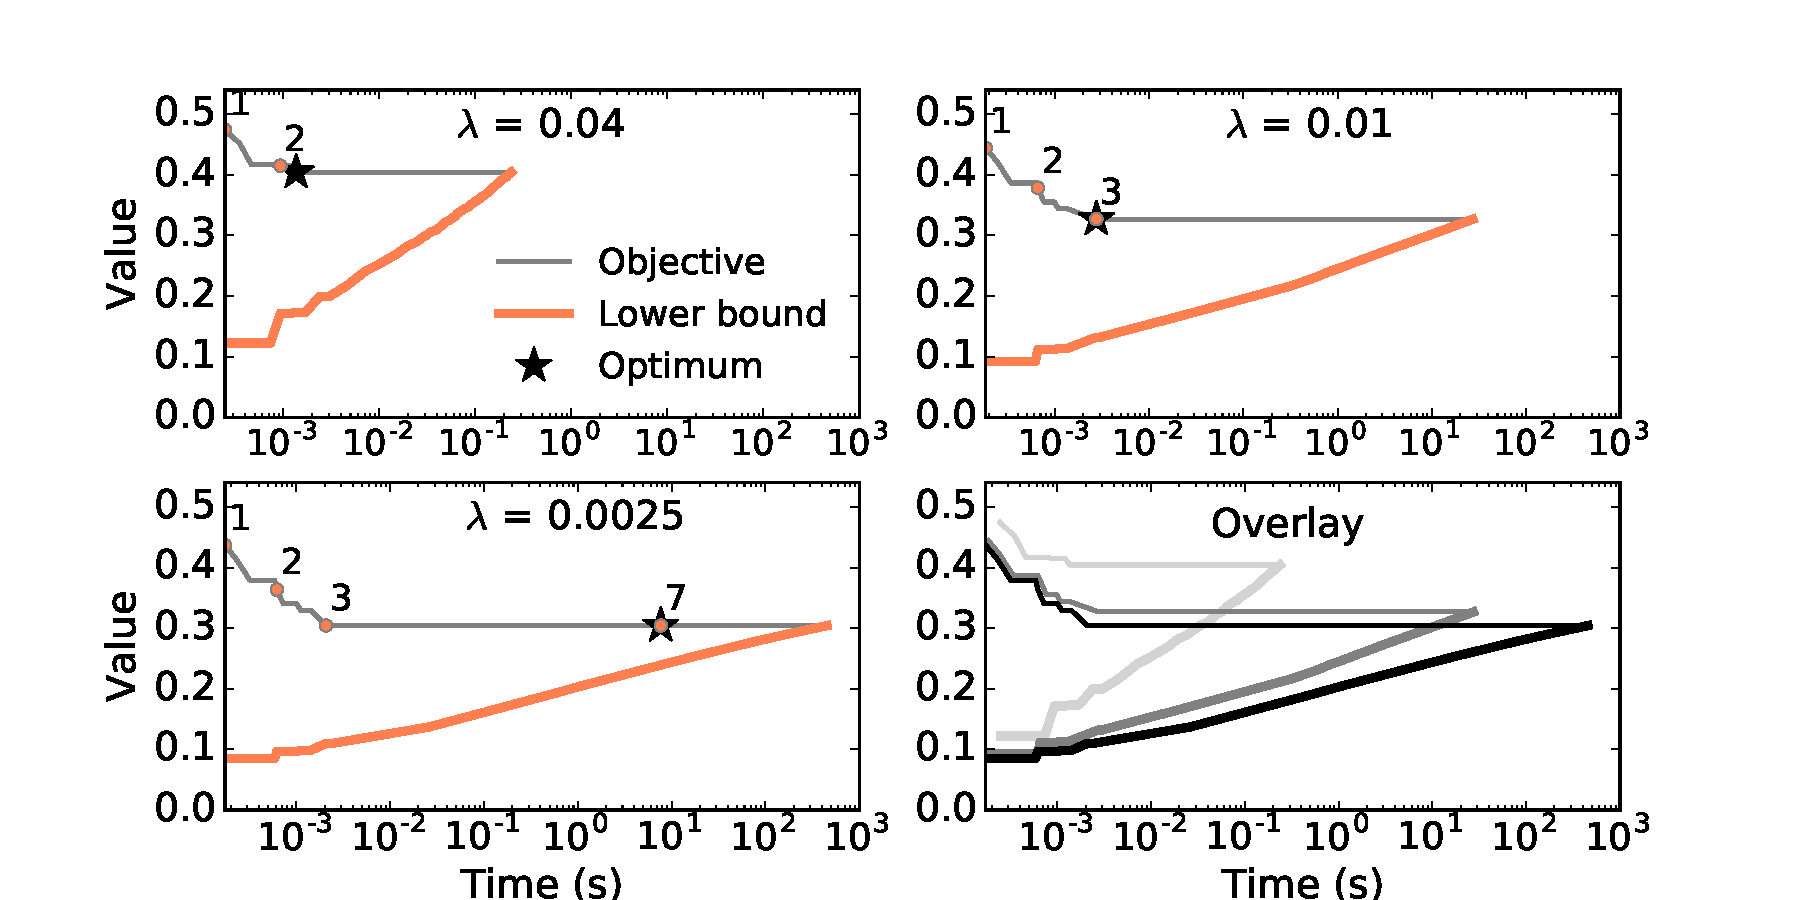
\includegraphics[trim={25mm 10mm 35mm 10mm},
width=0.45\textwidth]{figs/weapon_reg_small-execution.pdf}
\end{center}
\caption{Example CORELS execution traces (NYCLU).
%
Objective value (thin line) and lower bound (thick line) for CORELS.
%
Numbered points along the trace of the objective value
indicate when the length of the best known rule list changes
and are labeled by the new length.
%
For each value of~$\Reg$, a star marks the optimum
and the time at which it was achieved.
%
Bottom right: Overlay of the three traces.
}
\label{fig:weapon-reg-execution}
\end{figure}

\begin{figure}[t!]
\begin{center}
% left lower right upper
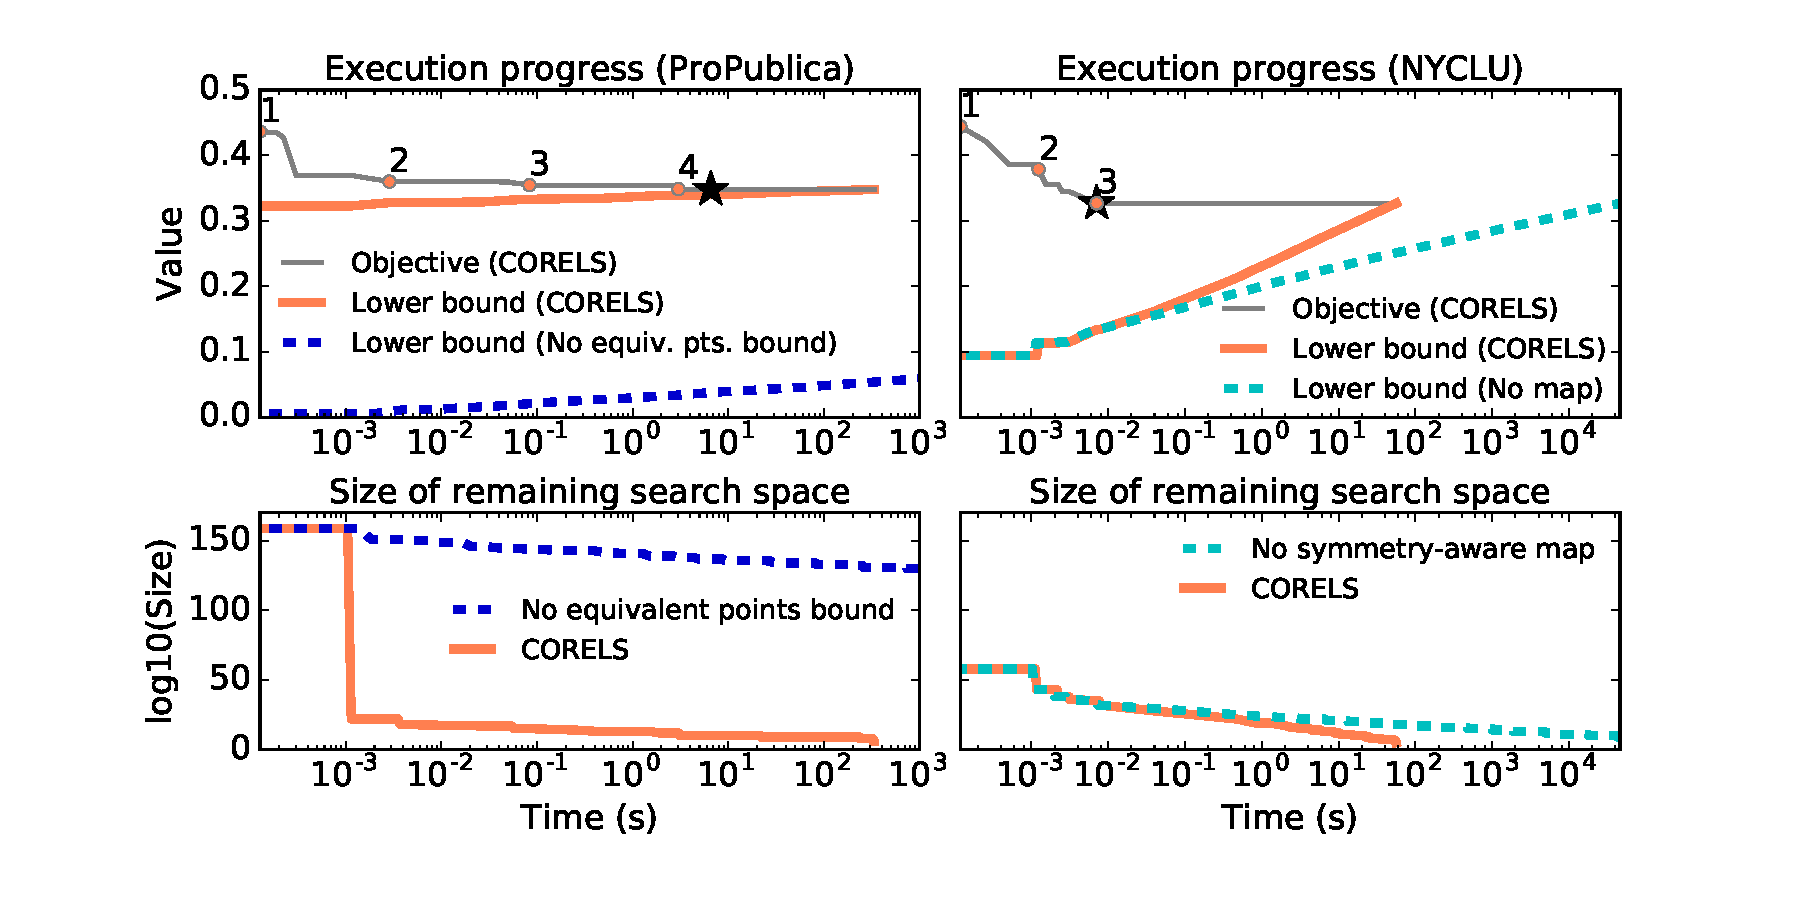
\includegraphics[trim={30mm 15mm 35mm 5mm}, width=0.45\textwidth]{figs/weapon_execution-remaining-space.pdf}
\end{center}
\vspace{-2mm}
\caption{Significant algorithm optimizations
for ProPublica (left) and NYCLU (right).
%
Top: Objective value (thin lines) and lower bound (thick lines) for CORELS,
as in Figure~\ref{fig:weapon-reg-execution},
and lower bound (dashes) from separate executions without
the equivalent points (left) and permutation (right) bounds.
%
Bottom: $\lfloor \log_{10} \Remaining(\CurrentObj, \Queue) \rfloor$,
where~$\Remaining(\CurrentObj, \Queue)$
is the upper bound on remaining search space size
(Theorem~\ref{thm:remaining-eval-fine}),
for CORELS (lines) and separate executions without selected bounds (dashes).
}
\label{fig:objective}
\end{figure}

As~$\Reg$ decreases, these times increase because the search problems become more difficult.
%
This is summarized by our observation that CORELS must evaluate longer prefixes:
across 10 cross-validation folds, the maximum evaluated prefix lengths are~6,
11, and~16 or~17, for ${\Reg = 0.04}$, $0.01$, and $0.025$, respectively.
%
As a consequence, our data structures grow in size: \eg
across 10 cross-validation folds, the mean number of queue elements are
1,900 (100), 170,000 (1,300), and 2,400,000 (170,000),
with standard deviations shown in parentheses,
for ${\Reg = 0.04}$, $0.01$, and $0.025$, respectively.


\textit{Algorithm optimizations:}
We determine the efficacy of each of our bounds and data structure optimizations.
%
In the remainder, we show results using the ProPublica dataset.
%
Table~\ref{tab:ablation} provides summary statistics for experiments using
the full CORELS implementation and variants that each remove a specific optimization.
%
Figure~\ref{fig:queue} presents a view of the same experiments, focusing
on three of our optimizations. These plots depict the number of
prefixes of a given length in the queue during the algorithm's execution.

\begin{table}[t!]
\centering
\resizebox{0.49\textwidth}{!}{
\begin{tabular}{l | c | c | c | c | c}
 & $t_\text{total}$ & $t_\text{opt}$ & $i_\text{total}$ & $Q_\text{max}$ & $K_\text{max}$ \\
Algorithm variant & (min) & (s) & ($\times 10^6$) & ($\times 10^6$) & \\
\hline
CORELS & 5.4 (1.6) & 8 (2) & 1.7 (0.4) & 1.3 (0.4) & 5-6 \\
BFS priority queue & 6.4 (2.0) & 34 (21) & 3.5 (1.4) & 2.6 (1.2) & 5-6 \\
No support bounds & 10.0 (3.3) & 12 (4) & 2.7 (0.8) & 2.2 (0.7) & 5-6 \\
No symmetry-aware map & 56.8 (22.3) & 21 (6) & 16.0 (5.9) & 14.5 (5.7) & 5-6 \\
No lookahead bound & 70.0 (22.0) & 8 (2) & 18.5 (5.9) & 17.1 (5.5) & 6-7 \\
No equivalent pts bound & $>$87 & $>$3744 & $>$1004 & $>$987 & $\ge$10
%No equivalent pts bound & 54.5 (44.6) & 2520 (2077) & 602.9 (492.2) & 593.0 (484.2) & 10-11
%folds that achieve min objective: 7
%num lower bound evals >= 1843354908
\end{tabular}
}
\vspace{4mm}
\caption{Per-component performance improvement.
%
The columns report total execution time,
time to optimum, number of queue insertions,
maximum queue size, and maximum evaluated prefix length.
%
The first row shows CORELS; subsequent rows show variants
that each remove a specific implementation optimization or bound.
%
We terminated each experiment in the last row once the size of the
trie reached ${10^9}$ nodes (each execution consumed $\sim$350GB RAM).
%
In all but the final row and column, we report means
(and standard deviations) over 10 cross-validation folds;
in the final row, we report the minimum values across folds.
}
\label{tab:ablation}
\end{table}

\begin{figure}[t!]
\begin{center}
% left lower right upper
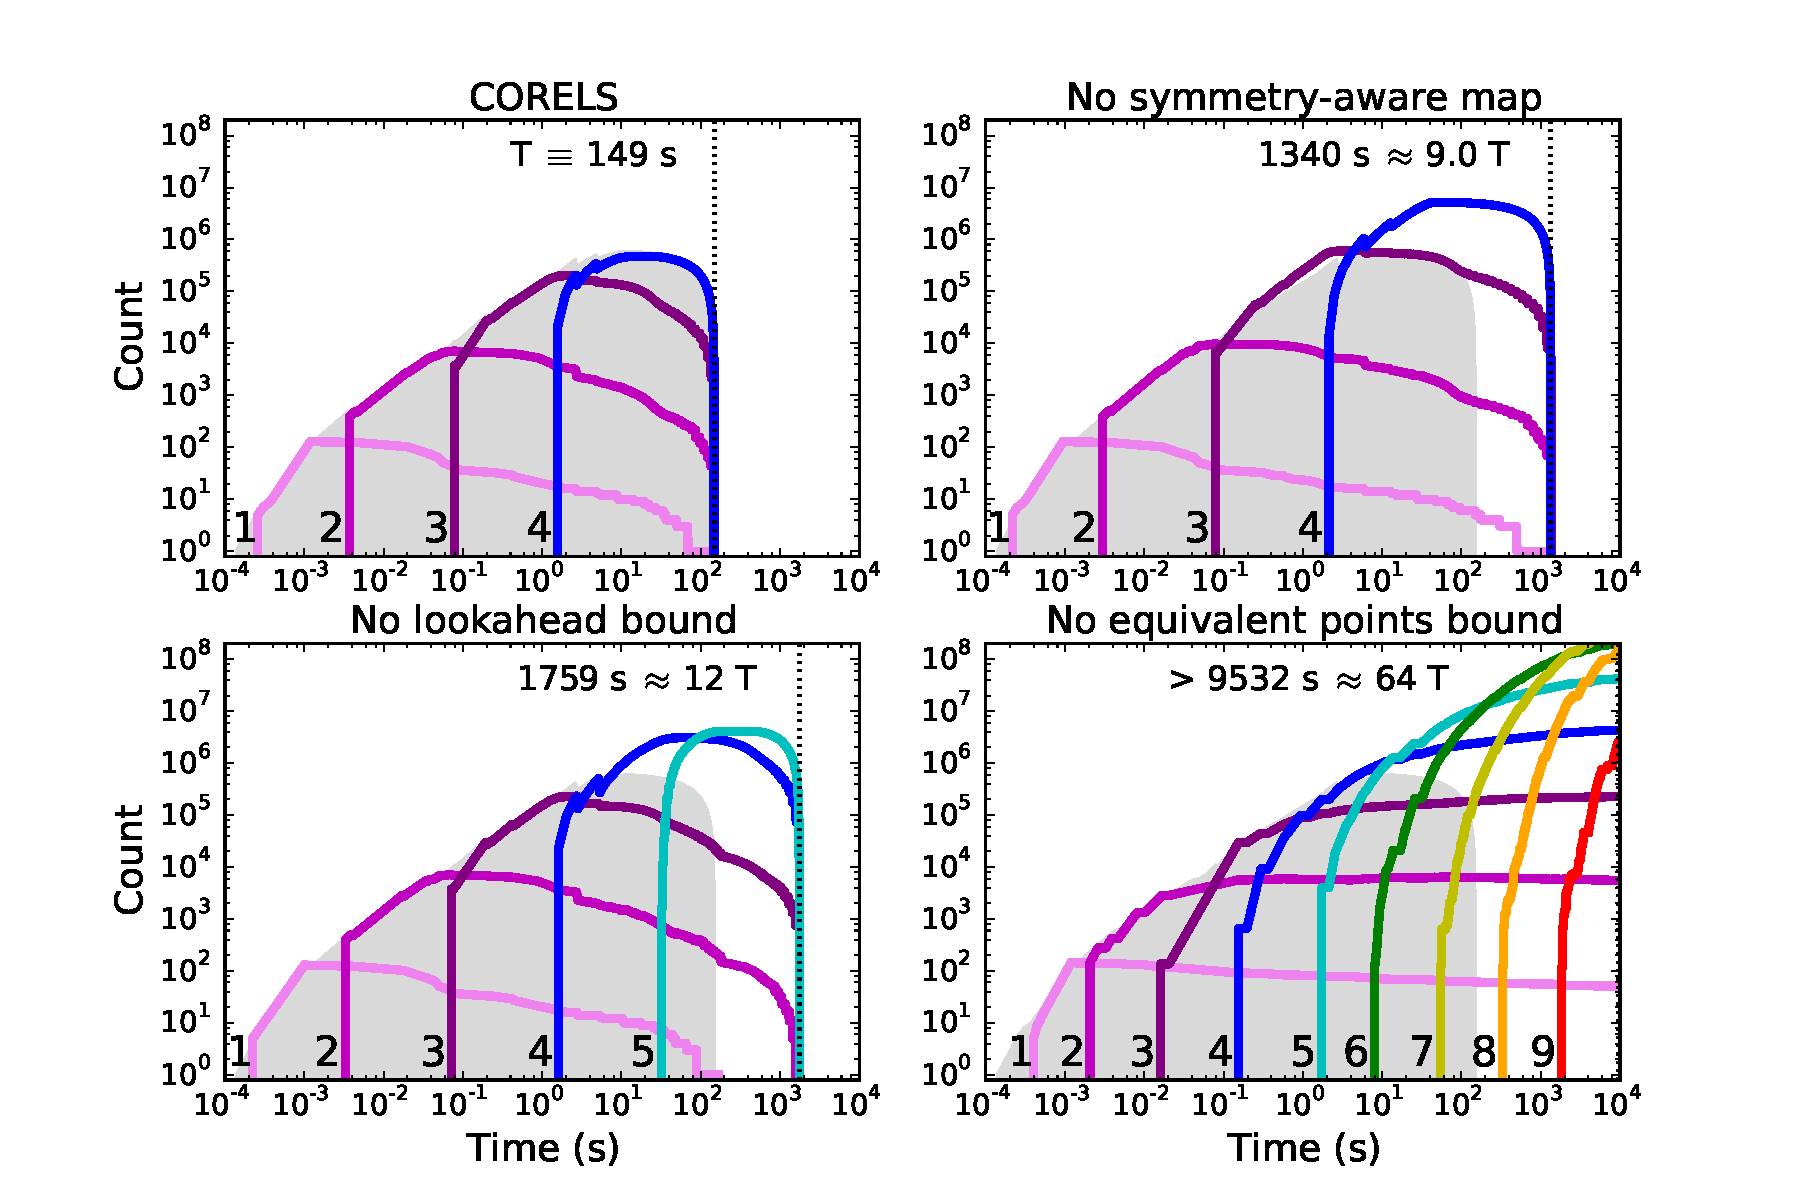
\includegraphics[trim={10mm 15mm 10mm 30mm},
width=0.45\textwidth]{figs/kdd_compas_ablation_small-queue.pdf}
\end{center}
\caption{Queue composition.
%
Numbers of prefixes in the queue (log scale), labeled and colored by length,
for CORELS (top left) and without three specific implementation optimizations or bounds.
%
The gray shading fills in the area beneath the total number of
queue elements for CORELS,
\ie the sum over all lengths in the top left figure.
%
For comparison, we replicate the same gray region in all subfigures.
}
\label{fig:queue}
\end{figure}


\textit{State space pruning:}
Figure~\ref{fig:objective} highlights the most significant
algorithm optimizations for our prediction problems,
using the ProPublica (left) and NYCLU (right) datasets.
%
On the left, for CORELS (solid lines),
the objective drops quickly, achieving the optimal value within 10~seconds.
%
CORELS certifies optimality in less than 6~minutes:
the objective lower bound steadily converges to the optimal objective (top)
as the search space shrinks (bottom).
%
In the same plots, we also show
a separate execution of CORELS without the equivalent points bound
(Theorem~\ref{thm:identical}) (dashes).
%
%After nearly 3~hours, this execution is still far from complete:
This execution is far from complete:
the lower bound is far from the optimum objective value (top)
and much of the search space remains unexplored (bottom).
%
On the right,
CORELS achieves the optimum objective in well under a second
and certifies optimality in less than a minute.
%
CORELS without the permutation bound (Corollary~\ref{thm:permutation}),
and thus the symmetry-aware map,
requires orders of magnitude more time to complete (dashes).

